\documentclass[12pt]{beamer}
\usepackage[latin1]{inputenc}
\usepackage{fancybox}
\usepackage{soul}
\usepackage{wasysym}
\usetheme{Warsaw}
\usepackage{graphicx}

\title[]{INF5050 \\ Protocols and routing in the internet}
\subtitle[]{Multiprotocol Label Switching (MPLS) \\ Generalized Multiprotocol Label Switching (GMPLS)}
\author{Mattias H{\aa}heim Johnsen -- mattiahj@ifi.uio.no}
\date{1. March 2013}

\begin{document}
\begin{frame}
    \titlepage
\end{frame}

\begin{frame}
  \frametitle{Introduction}
  \begin{itemize}
  \item What is MPLS?
  \item Why use MPLS?
  \item MPLS Fundamentals
  \item Traffic Engineering
  \item Quality of Service
  \item VPN
  \item GMPLS
  \item The future of MPLS
  \item Conclusion
  \item References and resources
  \end{itemize}
\end{frame}

\begin{frame}
  \frametitle{What is MPLS?}
  \begin{itemize}
    \item MPLS is a scalable data-carrying mechanism that directs data from one network node to the next based on short path labels rather than network addresses.
    \item Every network packet is assigned at least one label and packet-forwarding decisions are based on them exclusivly, rather than the content of the packets.
    \item Operates somewhere between layer 2 (data link layer) and layer 3 (network layer). Considered a "layer 2.5" protocol.
    \item Standardized by the IETF in 1996. Based on work done by Ipsilon Networks and Cisco.
  \end{itemize}
\end{frame}

\begin{frame}
  \frametitle{Why use MPLS?}
  \begin{itemize}
    \item Avoids complex lookups in the routing table.
    \item Allow core routers/networking devices to switch packets based on a simplified header.
    \item Create end-to-end circuits using any protocol over any IP capable transport medium.
    \item Provide a highly scalable mechanism that was topology driven rather than flow driven.
    \item Provides load-balancing functionality for traffic to utilize network bandwidth more efficiently.
    \item Remove the complexity and overhead of network managements (Assemble and reassemble IP packets).       
    \item Shortest path routing protocols like IS-IS and OSPF do not take capacity characteristics into account when making routing decisions. This leads to some network nodes being congested while others remain under-utilized.
  \end{itemize}
\end{frame}

\begin{frame}
  \frametitle{MPLS Fundamentals: Basic premise}
  \begin{itemize}
    \item By attaching a short fixed-length label to packets at the ingress to an MPLS domain these labels can be used to make forwarding decisions within that domain.
    \item Labels are assigned based on the concept of Forward Equivalence Classes. Packets belonging to the same FEC get the same label and generally travel by the same path across the network.
    \item !More about FEC
    \item These label switched paths may be explicitly routed if desired and can provide QoS when combined with Diff-Serv and Constraint-based routing.
    \item MPLS consists of a control plane and a forwarding plane that are decoupled/independent.    
    \end{itemize}
\end{frame}

\begin{frame}
  \frametitle{MPLS Fundamentals: Control Plane}
  \begin{itemize}
    \item The MPLS control plane is a collection of protocols that provide network level functionality in MPLS networks.
    \item These protocols are implemented as software processes that communicate with each other across node boundaries using message passing techniques.
    \begin{itemize}
      \item They facilitate the establishment of label switched paths in the MPLS networks by setting them up and tearing them down using signaling functions.
      \item The control plane distributes and manages network topology and resource availability information using a routing protocol
      \item For traffic engineering applications these protocols include the legacy IP routing and signaling protocols and extensions that provide the required functionality (ISIS-TE, OSPF-TE, RSVP-TE, CR-LDP, BGP).
    \end{itemize}
  \end{itemize}
\end{frame}

\begin{frame}
  \frametitle{MPLS Fundamentals: Forwarding Plane}
  \begin{itemize}
    \item The MPLS forwarding plane is the datapath user traffic is sent through. Also called the "data plane".
    \begin{itemize}
      \item The forwarding plane performs label swapping operations using lookup tables.
      \item Additionally it performs all miscellaneous packet treatment functions such as scheduling, queue management, rate shaping, policing and others.
      \item It is generally implemented in hardware due to the need for such operations to be done really quickly.
    \end{itemize}
  \end{itemize}
  \begin{figure}[h]
    \begin{center}
      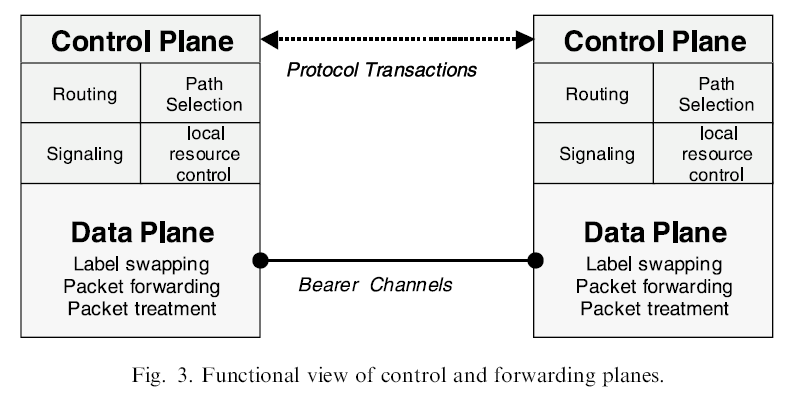
\includegraphics[scale=0.35]{label.png}
    \end{center}
  \end{figure}    
\end{frame}

\begin{frame}
  \frametitle{MPLS Fundamentals: MPLS Architecture 1}
  \begin{figure}[h]
    \begin{center}
      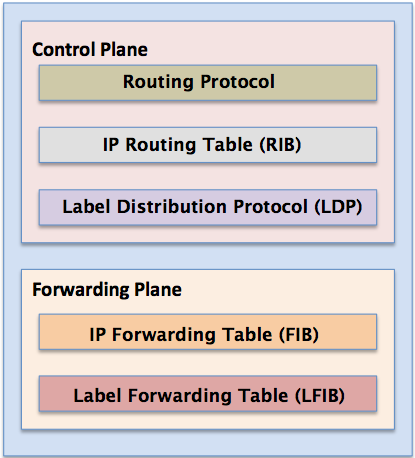
\includegraphics[scale=0.40]{mpls-arch.png}
    \end{center}
  \end{figure}    
\end{frame}

\begin{frame}
  \frametitle{MPLS Fundamentals: MPLS Architecture 2}
  \begin{figure}[h]
    \begin{center}
      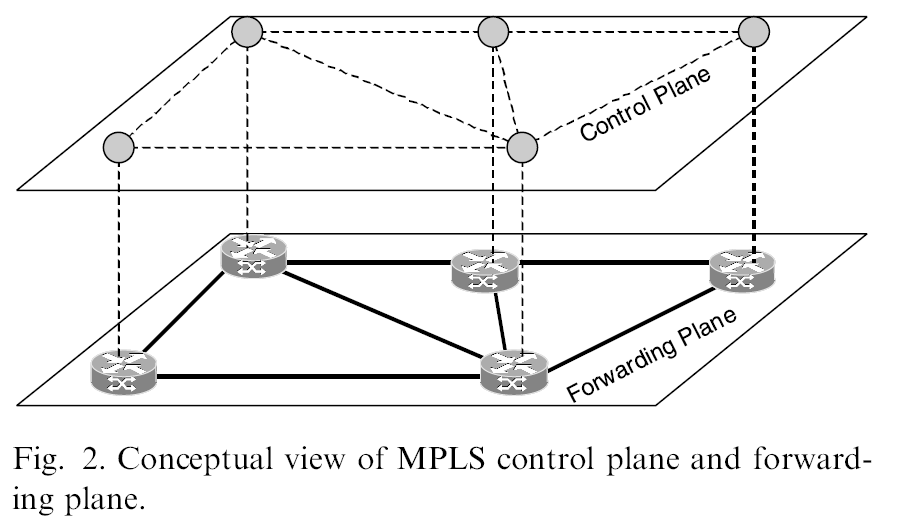
\includegraphics[scale=0.40]{separation.png}
    \end{center}
  \end{figure}
\end{frame}

\begin{frame}
  \frametitle{MPLS Fundamentals: Labels}
  \begin{itemize}
    \item an extra layer that "sits" between L2 and L3 layer known as header 2.5 (or "shim")
    \item don't need to lookup at the routing table, you use the label information to find the next hop
    \item creates a VPN rather than public networks
    \item isolates other traffics running on the network
  \end{itemize}
  \begin{figure}[h]
    \begin{center}
      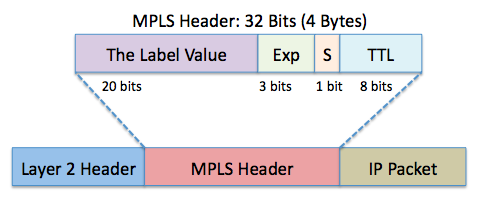
\includegraphics[scale=0.40]{header_mpls.png}
    \end{center}
  \end{figure}    
\end{frame}

\begin{frame}
  \frametitle{MPLS Fundamentals: The label header}
    Header information
    \begin{itemize}
      \item {\bf{Label value: }}the label itself for lookup in the MPLS forwarding table
      \item {\bf{EXP field: }}gives Diffserv support on the MPLS network and carry the IP precedence value from the IP packet.
      \item {\bf{Stack bit: }}Indicates the bottom of the MPLS header stack has been reached.
      \item {\bf{Time-To-Live: }}prevents loop and path tracing in the MPLS network. This value decrements with each hop and packet discards occur at a zero value.
    \end{itemize}       
\end{frame}

\begin{frame}
  \frametitle{MPLS Fundamentals: Label distribution}
  \begin{figure}
    \includegraphics<1>[scale=0.5]{animations/routeInit.png}
    \includegraphics<2>[scale=0.5]{animations/routereq1.png}
    \includegraphics<3>[scale=0.5]{animations/routereq2.png}
    \includegraphics<4>[scale=0.5]{animations/labeltable1.png}
    \includegraphics<5>[scale=0.5]{animations/labeltable2.png}
    \includegraphics<6>[scale=0.5]{animations/labeltable3.png}
    \includegraphics<7>[scale=0.5]{animations/labeltable4.png}
    \includegraphics<8>[scale=0.4]{animations/labeltable5.png}
    \includegraphics<9>[scale=0.4]{animations/path1.png}
    \includegraphics<10>[scale=0.4]{animations/path2.png}
    \includegraphics<11>[scale=0.4]{animations/path3.png}
    \caption{
      \only<1>{This is the initial phase}
      \only<2>{Ingress node makes a request to the nearest node for a given destination address}
      \only<3>{Route the message to the destination node}
      \only<4>{A label table is initialized with information that when it receives the given label id, it is for this router 47.1}
      \only<5>{Map its label id to the router that sent request}
      \only<6>{The router that receives the mapping data, adds it to its forwarding table and generates a "in" label}
      \only<7>{When finished, the egress node sends the mapping date of which label will be added }    
      \only<8>{When it has reached the Ingress node, it will map the given label for the given destination IP}
      \only<9>{Send message/packet to 47.1, the Ingress node makes a routing lookup and assigns the given label for the destination}
      \only<10>{When forwarded, you add label onto the packet, when it arrives to a node, it checks the label and replaces it to another one and forwards it}
      \only<11>{When reached to the egress node, it will then strip out the label and deliver to the specific destination}    
    }
  \end{figure}    
\end{frame}

\begin{frame}
  \frametitle{Traffic Engineering}
    Traffic engineering deals with performance optimization of operational ip networks. We want to transport ip packetsw in the most efficent reliable and expeditious manner possible through a given network.
    Avoid congestion and revocer from them when caused by poor resource allocation.
    Overutilized and congested resources with alternative viable paths that are under utilized.
    Generally: place traffic where the capacity exists to accommodate it.
    The ability to enable constraint-based routing in IP networks is one of the achievements of mpls that makes it particularly useful for traffic engineering.
\end{frame}

\begin{frame}
  \frametitle{Traffic Engineering: Process Model}
  %   Policy formulation phase
  %   Data acquisition phase
  %   analysis & characterization phase
  %   performance optimization phase
\end{frame}

\begin{frame}
  \frametitle{Traffic Engineering: Policy formulation phase}
  % Strategic or tactical
  %Ad-hoc approach
  %Optimize network performance by establishing and managing explicit LSP to adrress very specificnetwork performance problems.
  %For example: Create new LSPs to divert traffic away from congested network resources onto under-utilized alternatives.
  %Hybrid approaich: Use LSPs in some segments of the network while using interior gateway routing protocol metrics to control paths in other segments of the network.
\end{frame}

\begin{frame}
  \frametitle{Traffic Engineering: Data acquisition phase}
\end{frame}

\begin{frame}
  \frametitle{Traffic Engineering: Analysis and characterization phase}
\end{frame}

\begin{frame}
  \frametitle{Traffic Engineering: Performance optimization phase}
\end{frame}

\begin{frame}
  \frametitle{Traffic Engineering: What can MPLS bring to the table?}
\end{frame}

\begin{frame}
  \frametitle{Traffic Engineering: Diffserv}
  %A network architecture for classifying and managing network traffic and provide QoS on modern IP networks.
  %it is used to provide low-latency to critical network traffic. (Media, VOIP).
\end{frame}

\begin{frame}
  \frametitle{Traffic Engineering: Challenges and considerations}
  %Problem with computation of paths for LSPs subject to various types of constraints.
  %NP-complete problem
  %optimal partitioning and assignment of traffic to parallel LSPs between pairs of MPLS ingress and egress nodes.
  %Low visibility and lack of access into the MPLS cloud. How to monitor that your carrier is delivering the correct performance? 
  %Trace-route and ping no longer an option.
  %Probes are costly and difficult to maintain.
\end{frame}

\begin{frame}
  \frametitle{GMPLS: What is GMPLS?}
  \begin{itemize}
    \item A protocol suite extending MPLS to manage further classes of interfaces and switching technologies other than packet interfaces and switching, such as time division multiplex, layer-2 switch, wavelength switch and fiber-switch.
    \item GMPLS advocates and promotes explicit separation of the control plane from the underlying data/forwarding plane.
    \item Gives the ability to let products from different vendors to inter-operate at a control level in different types of switched transport networks.
  \end{itemize}
\end{frame}

\begin{frame}
  \frametitle{GMPLS: Origins}
  \begin{figure}[h]
    \begin{center}
      %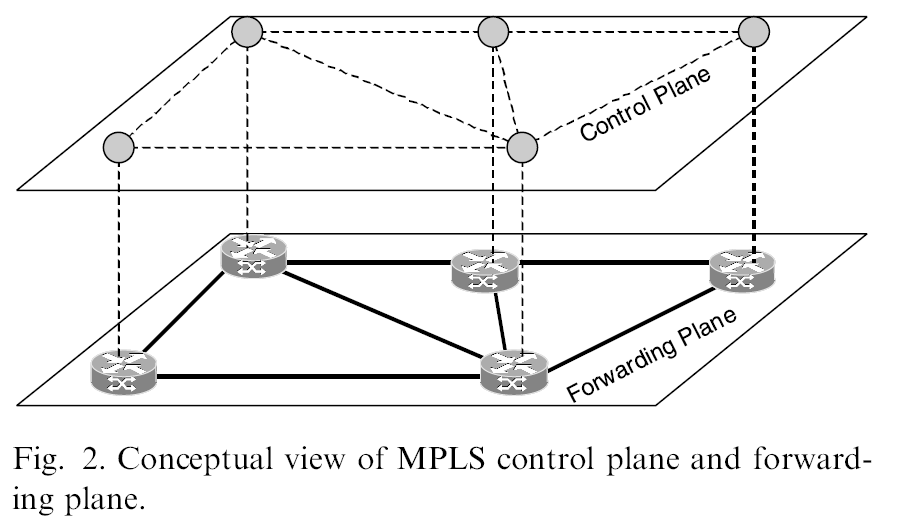
\includegraphics[scale=0.40]{separation.png}
    \end{center}
  \end{figure}
\end{frame}

\begin{frame}
  \frametitle{GMPLS: Why use GMPLS?}
  \begin{itemize}                             
    \item Allows new and innovative ways to inter-connect various technologies and different layers, without restricting the way individual layers interwork with each other. 
    \item It simplifies the design, deployment and operations management of heterogeneous networks consisting of an assortment of packet and circuit switched equipment from different manufacturers.
    \item consists of three main aspects: routing , signaling and link management.
    \item It also explicitly decouples the control channel from the transport or bearer channels.
    \item gives an important implications on the fault handling characteristics of the control plane.
    \item failure in the control plane does not imply failure of the transport plane.
  \end{itemize}
\end{frame}

\begin{frame}
  \frametitle{Conclusion}
  \begin{itemize}
    \item MPLS
    \item GMPLS
  \end{itemize}
\end{frame}

\begin{frame}
  \frametitle{References and resources}
  \begin{itemize}
    \item Generalized Multiprotocol Label Switching: An Overview of Signaling Enhancements and Recovery Techniques
          IEEE Communication Magazine, July 2001.
          A. Banerjee et. al. 
    \item Internet Traffic Engineering Using Multi-Protocol Label Switching (MPLS).
          Computer Networks 40, Elsevier, 2002
          D.O. Awduche and B. Jabbari. 
  \end{itemize}
\end{frame}

\end{document}
